\documentclass[whitelogo]{tudelft-report}
\usepackage{natbib}
\usepackage{changes}

\usepackage[justification=centering]{caption}

\begin{document}

%% Use Roman numerals for the page numbers of the title pages and table of
%% contents.
\frontmatter

%% Uncomment following 19 lines for a cover with a picture on the lower half only
%\title[tudelft-white]{Title}
%\subtitle[tudelft-cyan]{Optional subtitle}
%\author[tudelft-white]{J.\ Random Author}
%\affiliation{Technische Universiteit Delft}
%\coverimage{cover.jpg}
%\titleoffsetx{10cm}
%\titleoffsety{10cm}
%\afiloffsetx{1cm}
%\afiloffsety{18cm}
%\covertext[tudelft-white]{
%    \textbf{Cover Text} \\
%    possibly \\
%    spanning
%    multiple
%    lines
%    \vfill
%    ISBN 000-00-0000-000-0
%}
%\makecover

%% Uncomment following 16 lines for a cover with a picture on the lower half only
\title[tudelft-white]{Ubiquitous overlay}
\subtitle[tudelft-black]{Universal connectivity using imperfect hardware}
\author[tudelft-white]{Matouš Skála}
\affiliation{Technische Universiteit Delft}
\coverimage{network.jpg}


%\covertext[tudelft-white]{
%    \textbf{Cover Text} \\
%    possibly \\
%   spanning
%   multiple
%    lines
%   \vfill
%    ISBN 000-00-0000-000-0
%
\setpagecolor{tudelft-cyan}
\makecover[split]


%% Include an optional title page.
\begin{titlepage}


\begin{center}

%% Insert the TU Delft logo at the bottom of the page.

%% Print the title in cyan.
{\makeatletter
\largetitlestyle\fontsize{64}{94}\selectfont\@title
%\largetitlestyle\color{tudelft-cyan}\Huge\@title
\makeatother}

%% Print the optional subtitle in black.
{\makeatletter
\ifx\@subtitle\undefined\else
    \bigskip
   {\tudsffamily\fontsize{22}{32}\selectfont\@subtitle}
    %\titlefont\titleshape\LARGE\@subtitle
\fi
\makeatother}

\bigskip
\bigskip

by
%door

\bigskip
\bigskip

%% Print the name of the author.
{\makeatletter
%\largetitlefont\Large\bfseries\@author
\largetitlestyle\fontsize{26}{26}\selectfont\@author
\makeatother}

\bigskip
\bigskip

to obtain the degree of Master of Science
%ter verkrijging van de graad van Master of Science

at the Delft University of Technology,
%aan de Technische Universiteit Delft,

to be defended publicly on Tuesday January 1, 2013 at 10:00 AM.
%in het openbaar de verdedigen op dinsdag 1 januari om 10:00 uur.

\vfill

\begin{tabular}{lll}
    Student number: & 4893964 \\
    Project duration: & \multicolumn{2}{l}{November 15, 2019 -- June 30, 2020} \\
    Thesis committee: & Dr.ir. J.A. Pouwelse, & TU Delft, supervisor \\
        & ?, & TU Delft \\
        & ?, & TU Delft
\end{tabular}
%% Only include the following lines if confidentiality is applicable.

\bigskip
\bigskip
%\emph{This thesis is confidential and cannot be made public until December 31, 2013.}
%\emph{Op dit verslag is geheimhouding van toepassing tot en met 31 december 2013.}

\bigskip
\bigskip
An electronic version of this thesis is available at \url{http://repository.tudelft.nl/}.
%\\[1cm]

%\centering{
\includegraphics{cover/logo_black}}


\end{center}

\begin{tikzpicture}[remember picture, overlay]
    \node at (current page.south)[anchor=south,inner sep=0pt]{
        
\includegraphics{cover/logo_black}
    };
\end{tikzpicture}

\end{titlepage}



\chapter*{Preface}
\setheader{Preface}

When I was choosing my thesis topic, I originally came up with an idea of designing a decentralized social network. After realizing how ambitious that goal was, I later decided to focus on more fundamental issues first and create a library that would allow for building any decentralized applications, running purely on an overlay network consisting of smartphones. Rather than reinventing the wheel, I took inspiration from an existing networking library developed at TU Delft over the last decade and created its wire-compatible implementation in Kotlin. Interestingly, in the end, I have even implemented a trivial social network to demonstrate the usage of the library, returning back to the original idea.

I would like to thank my supervisor Johan Pouwelse for an endless stream of fresh ideas and valuable feedback, and to PhD students of the Delft Blockchain Lab for numerous coffee meetings and for serving me as a walking documentation of the existing codebase.

\begin{flushright}
{\makeatletter\itshape
    \@author \\
    Prague, August 2020
\makeatother}
\end{flushright}



\tableofcontents

%% Use Arabic numerals for the page numbers of the chapters.
\mainmatter

\chapter{Introduction}

// TODO: rewrite introduction

The Internet was created with the idea that any two computers connected to the common network should be able to communicate with each other. In the Internet Protocol, each computer gets assigned an address which is subsequently used for packet routing. The most common version of the protocol, IPv4, uses a 32-byte address space which is not enough to uniquely identify all devices on the planet. To deal with IPv4 address exhaustion, internet providers were forced to deploy different types of \textit{Network Address Translation (NAT)} which allows a single address to be shared across multiple devices.

Another issue appeared with the rise of portable computers and smartphones. IPv4 addresses are dependent on the physical location and can not be considered stable user identifiers. There has been several proposals including Mobile IP, IPSec, and IPv6 to improve the usability and security of the Internet Protocol. However, none of them have been widely deployed yet or address all known issues.

% TODO: client-server model, but recently trend is decentralization

This thesis proposes and implements a decentralized protocol for peer to peer communication between any two devices. It is implemented in form of a Kotlin library which can be used on desktop, smartphones, tablets, and IoT devices. This library can be used to deploy a truly ubiquitous network overlay which is available anytime and everywhere. The protocol allows any two devices to establish a direct connection by taking advantage of NAT traversal techniques to connect peers behind NATs. When the Internet connection is not available and peers are located in proximity, the connection can be established using Bluetooth Low Energy. Peers are addressed by their public keys and their physical addresses on lower layers are abstracted away.

The protocol makes best effort to connect peers behind NATs. However, in case the connection is not possible, it resorts to a relay protocol. Bandwidth accounting prevents misusing the relay servers and provides incentive for relay operators. The protocol is completely decentralized and does not rely on any central entity.

%This also allows to route messages over multiple transports. For example, a message can be send over Bluetooth and delivered to a user connected over the Internet by using another device a relay.

To show one of many practical use cases of the protocol, a simple chat messaging application is implemented on top of it. It allows two users to exchange identities in a secure way to prevent MITM attack. Then they can transfer not only text messages, but also images and videos, to demonstrate a binary file transfer.

Compared to the state of the art solutions, the proposed library combines both nearby and Internet connectivity, does not require any central server, works on a variety of devices, and is completely open source.

Finally, the protocol performance is experimentally evaluated with multiple Android devices connected to different Wi-Fi and carrier networks and running a stress test over the period of 24 hours.

\iffalse
\fi

\chapter{Problem Description}

%\section{Ubiquitous Overlay Network}

\section{End-to-end Principle Challenged}

\section{Net Neturality Under Attack}

\section{In Quest of Trustworthy Communication}

\section{Re-decentralization of Internet Infrastructure}

% history of internet, IPv4
% address exhaustion, mobility

% NAT breaks end-to-end principle
% solutions:
% - IPv6
% - Mobile IP
% - IPSec
% IPv6 still not widely deployed
% - TU preparing for IPv6 since 2012
% - not available on any cellular network in NL

% motivation for decentralized internet
% problems with current internet:
% - censorship
% - data in control of big companies
% we need building blocks to disrupt centralized services
% data in controls of users
% first steps: connectivity, data availability, privacy
% mention blockchain as enabler of permissionless economic activity

% ubiquitous overlay
% - peer to peer connectivity over the Internet
% - off-grid communication without internet access

% research question: How to establish a secure connection between two smartphone devices without using a central server?


\chapter{State of the Art}

\section{Network Address Translation}

\subsection{NAT Classification}

% Mapping: Endpoint-Independent, Address-Dependent, Address- and Port-Dependend
% Filtering: Endpoint-Independent, Address-Dependent, Address- and Port-Dependend

% Most common implementations (TODO: show table with mapping and filtering behavior):
% - Full Cone NAT
% - Restricted Cone NAT
% - Port Restricted Cone NAT
% - Symmetric NAT

% Hairpinning

% NAT detection in STUN

\subsection{Carrier Grade NAT}

\subsection{Port Forwarding}

% mention protocols for port forwarding configuration: UPnP-IGD, NAT-PMP, PCP
% usually not enabled by default, not enabled in carrier networks

\section{NAT Traversal}

\subsection{Session Traversal Utilities for NAT (STUN)}

\subsection{Traversal Using Relays around NAT (TURN)}

\subsection{Interactive Connectivity Establishment (ICE)}

% \subsection{ICMP Hole Punching}

\subsection{Symmetric NAT Traversal}

\section{Nearby Communication}

Modern smartphone devices come equipped with several wireless communication standards that can potentially be used for communication with other nearby devices. It is desirable to use such a technology when multiple devices in proximity want to communicate with each other when there is no reliable Internet infrastructure available. These technologies can be also preferred over the Internet in case of censorship and privacy concerns, as has been shown during numerious occasions such as Hong Kong protests. From the user experience perspective, it is desired that the device discovery and connection establishment does not require any user interaction besides the one required by the application use case. However, this is often difficult to achieve in the security model of smartphone operating systems, which try to protect users by enforcing a system UI for any sensitive operations, as shown in Figure \ref{system_ui}.

\begin{figure}
    \centering
    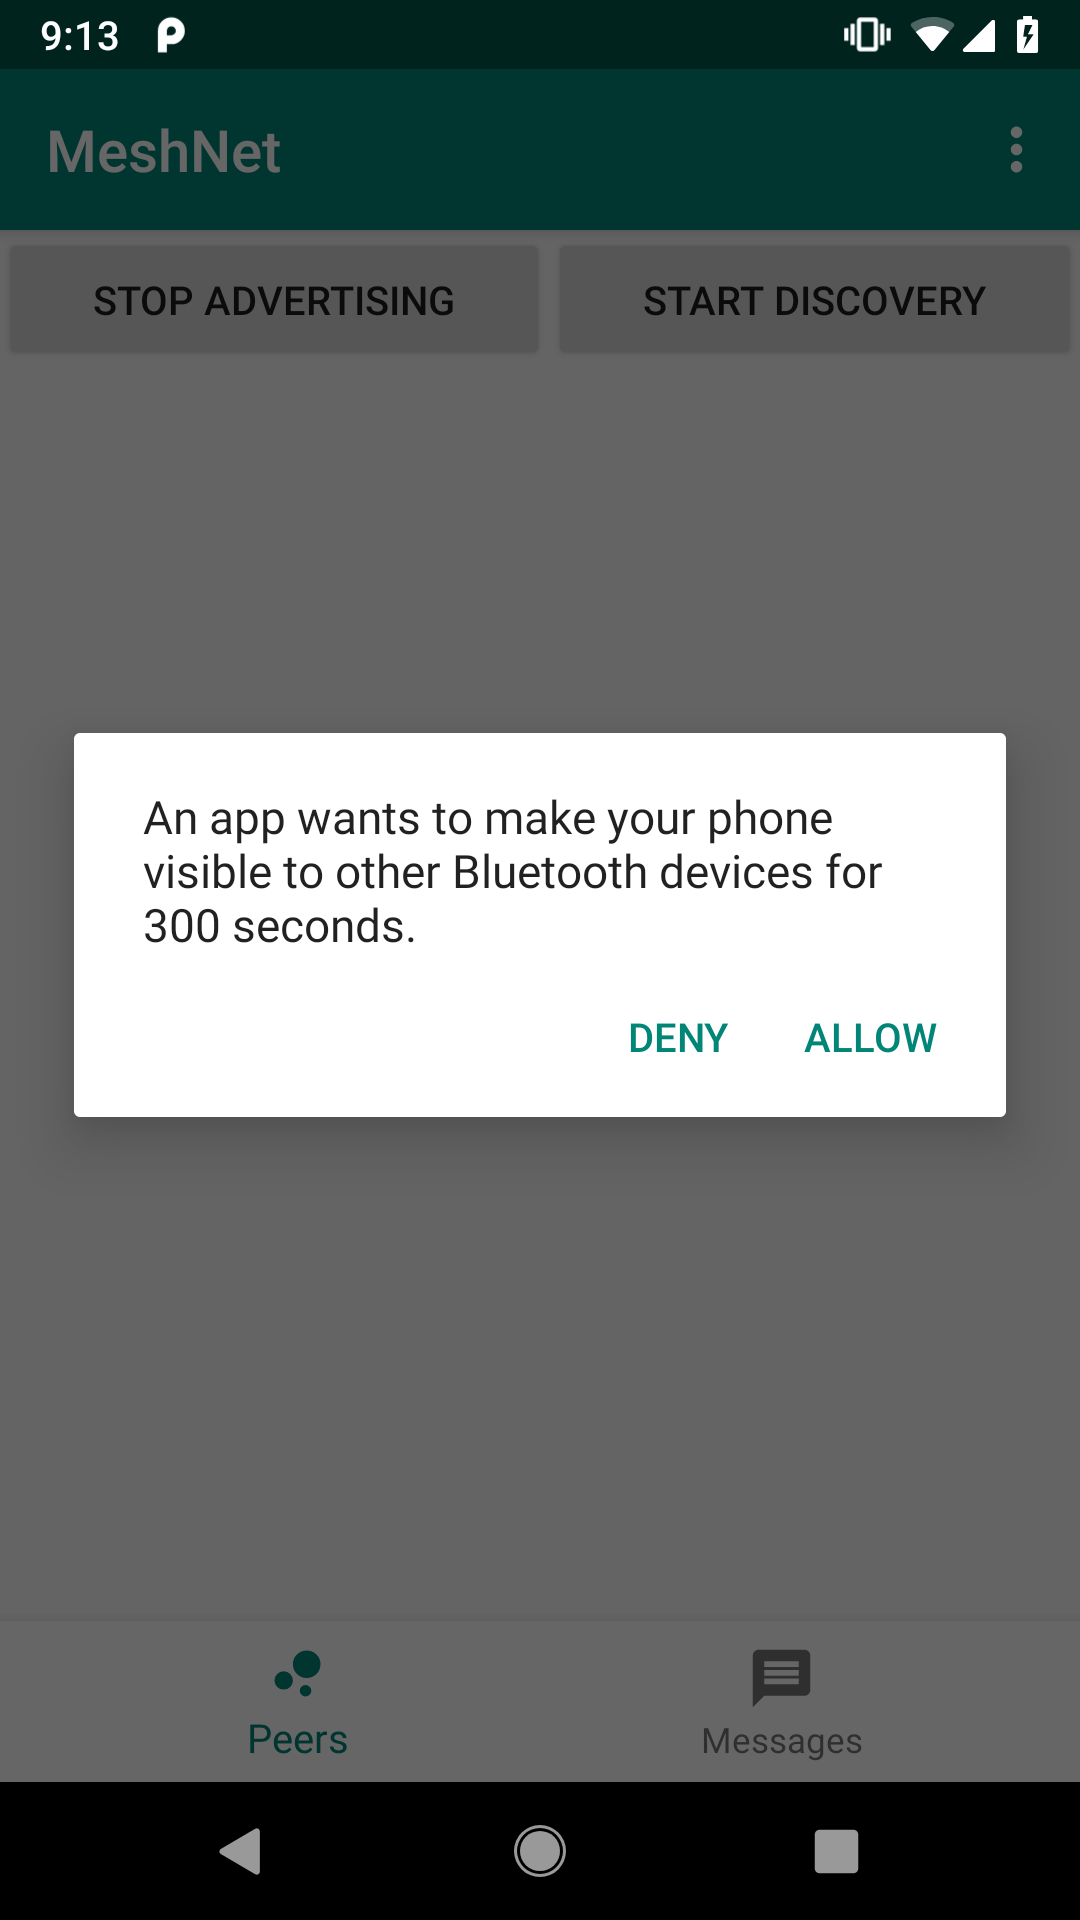
\includegraphics[width=0.32\textwidth]{screens/dialog_bluetooth-discovery}
    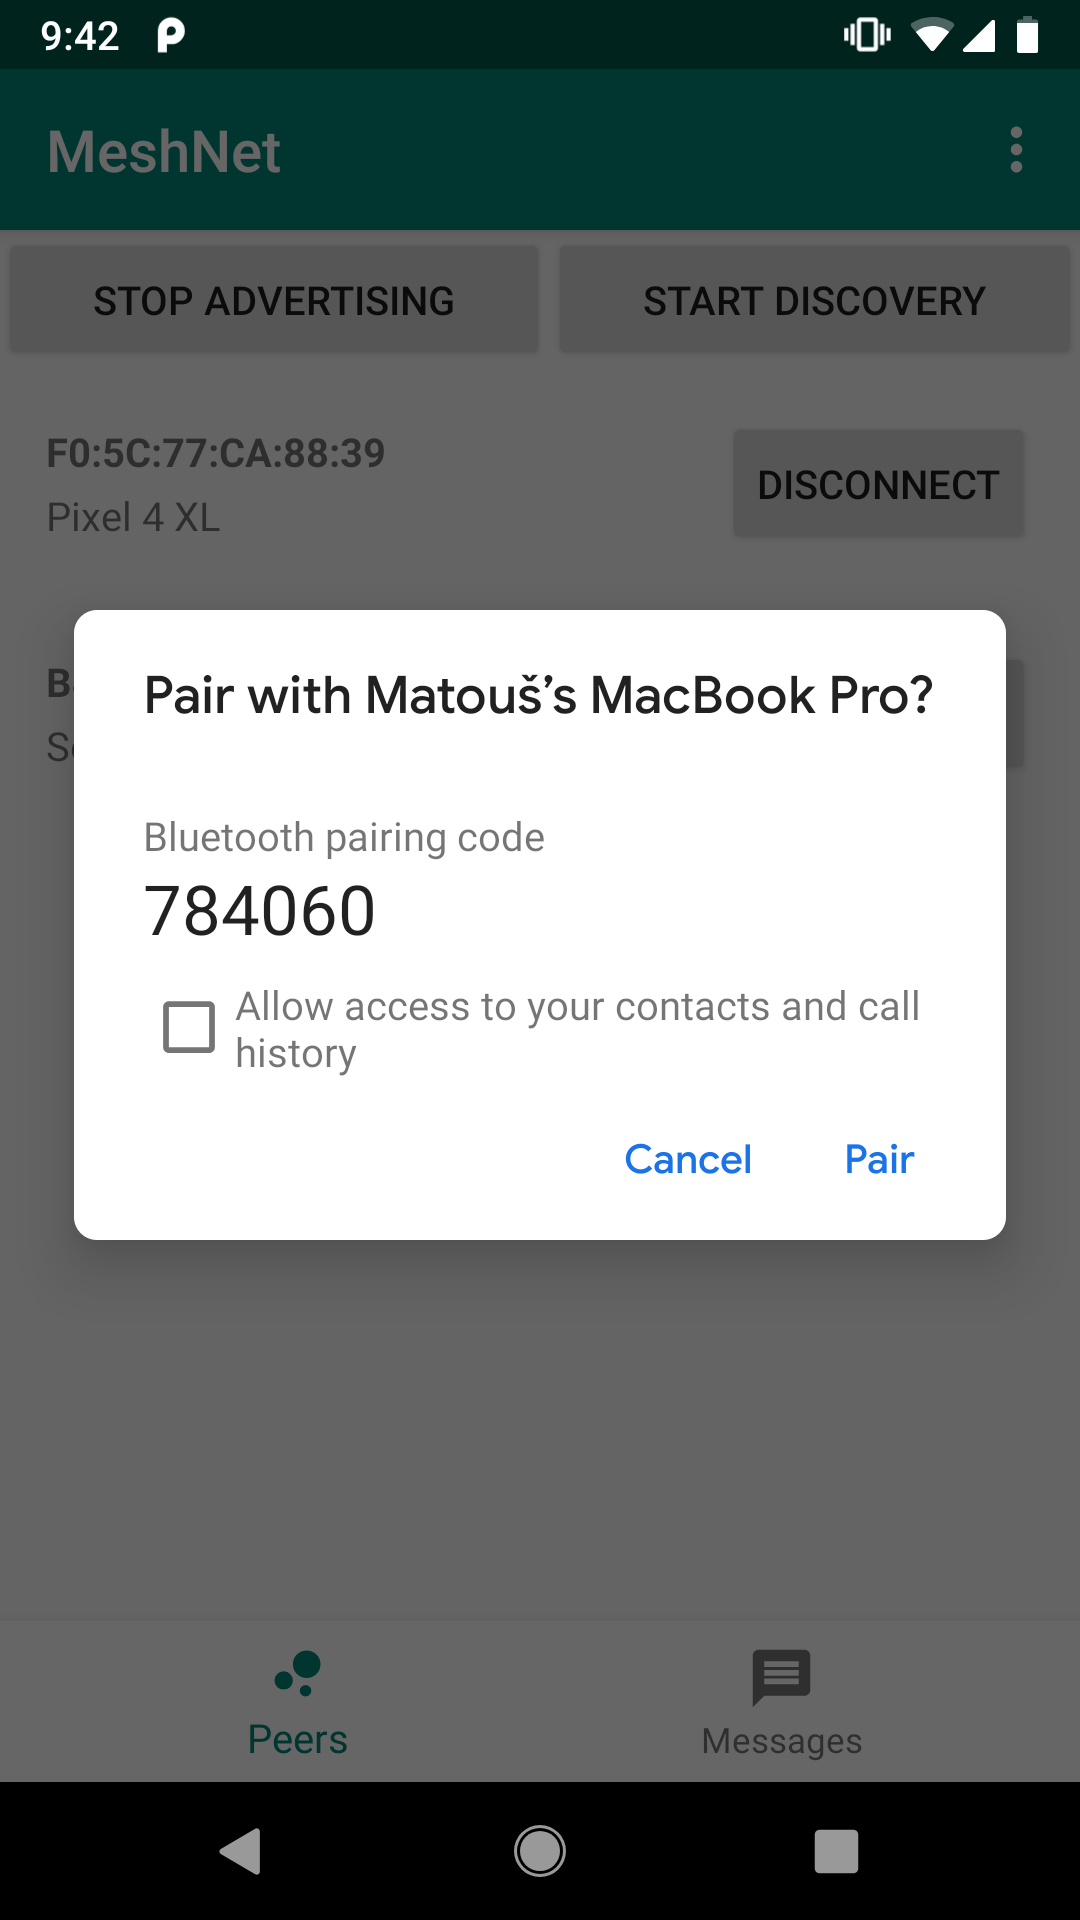
\includegraphics[width=0.32\textwidth]{screens/dialog_bluetooth-pairing}
    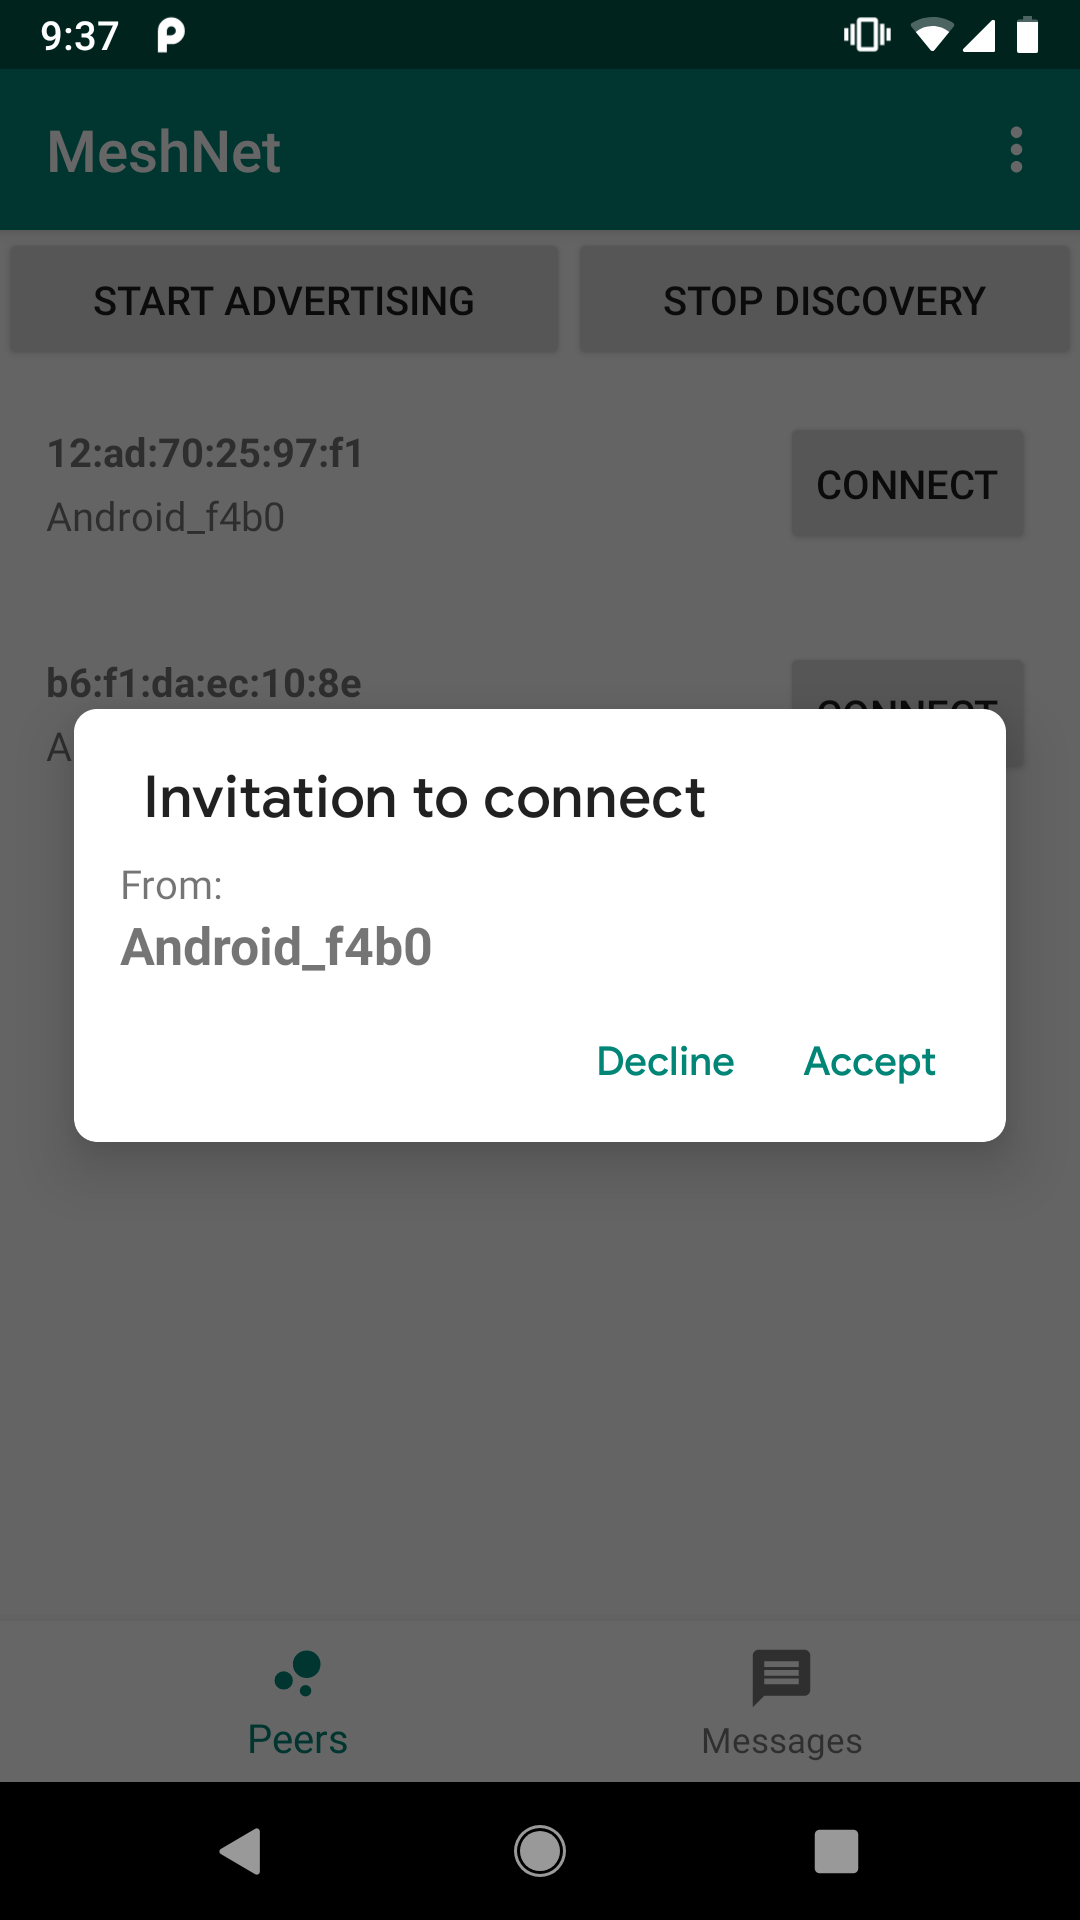
\includegraphics[width=0.32\textwidth]{screens/dialog_wifi-direct}
    \caption{The system UI for enabling Bluetooth discovery, accepting an incoming Bluetooth pairing request, and accepting an incoming Wi-Fi Direct connection on Android 9}
    \label{system_ui}
\end{figure}

% TODO: add screenshots of Bluetooth enable discovery, pairing dialog, WiFi direct dialog

\subsection{Bluetooth}

The oldest and the most battle-tested technology for nearby connectivity is Bluetooth, which has been in development for more then 20 years. The common flow for Bluetooth usage is to first force the user to \textit{pair} (or \textit{bond}) two devices. The device A first needs to manually be set as \textit{discoverable}, usually for a limited time period. The device B then performs a scan to discover nearby devices. The device B can then send a pairing request to the selected device. Then a pairing code is displayed and once both users accept the pairing request, the devices are paired.

Only after that, a secure \textit{Radio frequency communication (RFCOMM)} channel can be established. The pairing process requires user interaction, which degrades the user experience in certain applications when authentication is performed on the application level. While it is possible to establish an \textit{insecure} RFCOMM channel if the MAC address of the other device is known, the user of the other device still needs to manually set it to be discoverable.

\subsection{Bluetooth Low Energy}

% TODO: cite specification

\textit{Bluetooth Low Energy (BLE)} \cite{blebook} was introduced in 2010 as part of the Bluetooth 4.0 specification. It is a completely different communication protocol incompatible with the classic Bluetooth. BLE offers considerably decreased power consumption with a similar communication range and slightly lower bandwidth. It was originally intended to support an infrequent low-power communication with wearables, healthcare accessories, or smart home appliances. However, while it is not a primary use case, it could also be potentially used for low-bandwidth peer-to-peer communication between smartphone devices.

It is notable that once an application is granted a Bluetooth permission, it can fully control BLE APIs without any user interaction, which opens up doors for a range of many different applications.

% use cases: mesh networks
% upper physical throughput: 1 Mbps (modulation rate)

\subsection{Wi-Fi Direct}

\subsection{Wi-Fi Aware}


\subsection{Support in Operating Systems}

\begin{table}
    \centering
    \begin{tabular}{ | l | l | l | l | l | }
      \hline
      \textbf{Technology} & \textbf{Android} & \textbf{iOS} & \textbf{Throughput} & \textbf{Range} \\
      \hline
      Bluetooth & 2.0+ & 5.0+ & 2 Mbps & $\sim$40 m \\
      \hline
      BLE Advertising & 4.3+ & 6.0+ & \multirow{3}{*}{0.3 Mbps} & \multirow{3}{*}{$\sim$100 m} \\
      BLE GATT & 5.0+ & 6.0+ & &  \\
      BLE L2CAP & 10.0+ & 11.0+ & &  \\
      \hline
      Wi-Fi Direct & 4.0+ & N/A & \multirow{2}{*}{250 Mbps} & \multirow{2}{*}{$\sim$200 m} \\
      Wi-Fi Aware & 8.0+ & N/A & & \\
      \hline
    \end{tabular}
    \caption{The comparison of properties of the most common wireless communication technologies and their support in smarphone operating systems
    }
    \label{wirelesstech_table}
  \end{table}




% technologies available on smartphones:
% - Bluetooth, BLE, WiFi Direct, WiFi Aware
% infrastructureless communication

% Bluetooth Classic
% - requires the device to be discoverable - user interaction
% - no interoperability between iOS and Android
% Bluetooth Low Energy
% - energy efficient, does not require pairing, but lower bandwidth
% - API on Android very low level, error-prone to use
% - role simultaneity – master and slave at the same time


\section{P2P Communication Libraries}

\subsection{libp2p}

\subsection{Nearby Connections API}

\subsection{MultipeerConnectivity}

\subsection{Bridgefy SDK}

\subsection{Berty Protocol}

\subsection{IPv8}

\chapter{Design}

%\section{NAT Detection}

\section{NAT Traversal with Peer Introductions}


%\begin{figure}
%    \centering
%    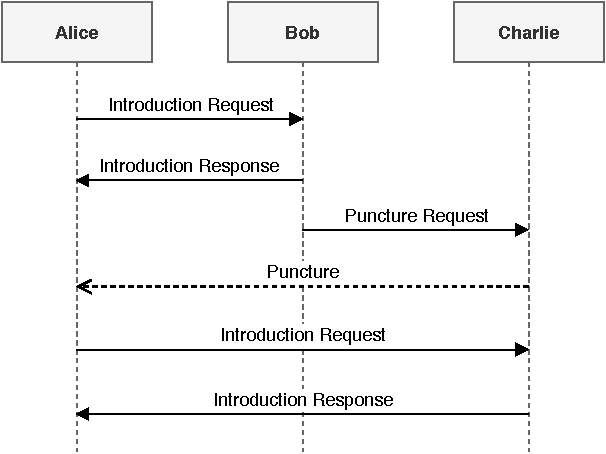
\includegraphics[width=0.6\textwidth]{diagrams/uml_peer-introduction}
%    \caption{Peer discovery mechanism with NAT puncturing}
%\end{figure}

%\section{Port Forwarding}

%\section{Symmetric NAT Traversal}

% \section{Network Service Discovery}

\clearpage

\section{P2P Communication with Nearby Devices}

\subsection{Introduction to Bluetooth Low Energy}

In this section, we introduce the most important Bluetooth Low Energy concepts defined in the Bluetooth specification \cite{bluetooth51spec}. This background knowledge is fundamental for understanding the subsequent sections. In principle, there are two methods that BLE devices can use for communication: using connectionless \textit{broadcasting}, or by establishing \textit{connections}.

\subsubsection{Broadcasting}

BLE advertising packets are used to broadcast data to multiple peers at the same time. Other devices can run a \textit{scanning} procedure to read advertisement packets. Each advertisement packet can carry 31-byte payload to describe its capabilities and or any other custom information. Optionally, the scanning device can request a \textit{scan response} from the advertiser, in which the advertiser can send an additional 31-byte payload. That means 62 bytes in total can be transmitted using the broadcasting mechanism. It is important to note that this is unidirectional data transfer and the broadcaster has no way to specify who can receive those packets, or receive any acknowledgements.

\subsubsection{Connections}

An advertising packet can be marked as \textit{connectable}. In that case, if data have to be transferred bidirectionally or more than 62 bytes are required, a connection between two devices can be established.

Devices in BLE can act in two roles: \textit{centrals} and \textit{peripherals}. A central repatedly scans for advertising packets broadcasted by peripherals and when needed, it initiates a connection. A peripheral then periodically broadcasts advertising packets and accepts incoming connections. There are no restrictions on connection limits imposed by the specification. Since Bluetooth 4.1, a single device can act both as a central and peripheral at the same time, and it can also be connected to multiple centrals/peripherals.

\subsubsection{Address Types}

The BLE protocol stack differentiates between two types of addresses. The \textit{public address} is a standard IEEE-assigned MAC address that uniquely identifies the hardware device. Since all BLE packets include a device address, it would be possible to track device movement by adversial scanners. BLE addresses this issue by using a \textit{random address} for any communication. This address is generated using the combination of a device \textit{identity resolving key} and a random number, and it can be changed often, even during the lifetime of a connection.

\subsection{BLE Protocol Stack}

The BLE standard is composed of several protocols which form the BLE stack visualized in Figure \ref{ble_stack}. The stack is split in two parts: a \textit{controller} and a \textit{host}. The controller is usually implemented in hardware, while the host is a part of the operating system. Both parts communicate over the \textit{Host Controller Interface (HCI)}. Even though the applications usually communicate only with the highest layers, it is worth to understand how all layers of the stack fit together. In this section, we describe the responsibilities and mechanics of each protocol.

\begin{figure}
    \centering
    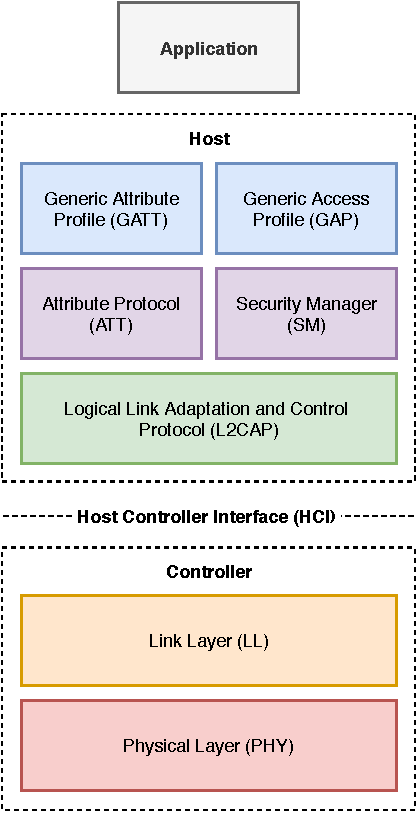
\includegraphics[width=0.40\textwidth]{diagrams/ble-stack}
    \caption{Bluetooth Low Energy Protocol Stack \cite{blebook}}
    \label{ble_stack}
\end{figure}

\subsubsection{Logical Link Control and Adaptation Protocol (L2CAP)}

On the lowest layer in the host, L2CAP is responsible for multiplexing and splitting data from higher-level protocols (ATT and GAP) into 27-byte data packets. These are then forwarded to the Link Layer and transmitted over the Physical Layer implemented in the Bluetooth radio. Starting with Bluetooth 4.1, the applications can communicate over L2CAP directly. User-defines channels allow for higher-throughput data transfer without the additional complexity added by ATT.

% \subsubsection{Security Manager (SM)}

\subsubsection{Generic Access Profile (GAP)}
// TODO

\subsubsection{Attribute Protocol (ATT)}
ATT is a client-server protocol for reading and writing attributes. It is strict about sequential operation. If a request is pending, no further requests should be sent until the response is received, otherwise they are discarded. Attributes are stored under attribute handles defined by UUIDs. Various operations are defined by the protocol. Apart from the standard configuraiton, read and write, queued write is supporte to write data longer than a single packet. If a client wants to be notified about handle changes, it can subscribe to handle value notifications or indications. Both allow the server to notify the clients whenever a value changes, but in case of indication, the client should respond with ack packet to confirm it has received the indication.

\subsubsection{Generic Attribute Profile (GATT)}

The Generic Attribute Profile defines how to exchange data between devices. It uses ATT as a transport protocol. The data are organized hierarchically in \textit{services} which contain groups of related data called \textit{characteristics}, which can be further specified using \textit{descriptors}.

GATT is a client–server protocol and it follows the same principles as ATT. A client sends requests to the server and receives responses or server-initiated updates. The server is responsible for storing data written by the client and responding to read requests. It is important to mention that the client and server roles in GATT are independent of the roles defined by GAP. Both a peripheral and a central can take the role of a client or a server, or even both at the same time.

%\subsection{Using Bluetooth Low Energy for P2P Communication}

%\subsection{Bluetooth Device Address}

\subsection{BLE Communication Architecture}

As mentioned earlier, the primary purpose of BLE was to enable exchange of information with peripheral devices. However, as it is currently the most universal way for nearby communication on mobile devices that does not require any user interaction, it is potentially suitable for any type of communication. Since Android 5.0, it is possible to create a custom GATT server which allows two Android devices to communicate with each other over BLE. We now proceed to designing a system architecture for P2P communication using BLE. The overall high-level architecture of data flow is shown in Figure \ref{ble_architecture}.

\begin{figure}
    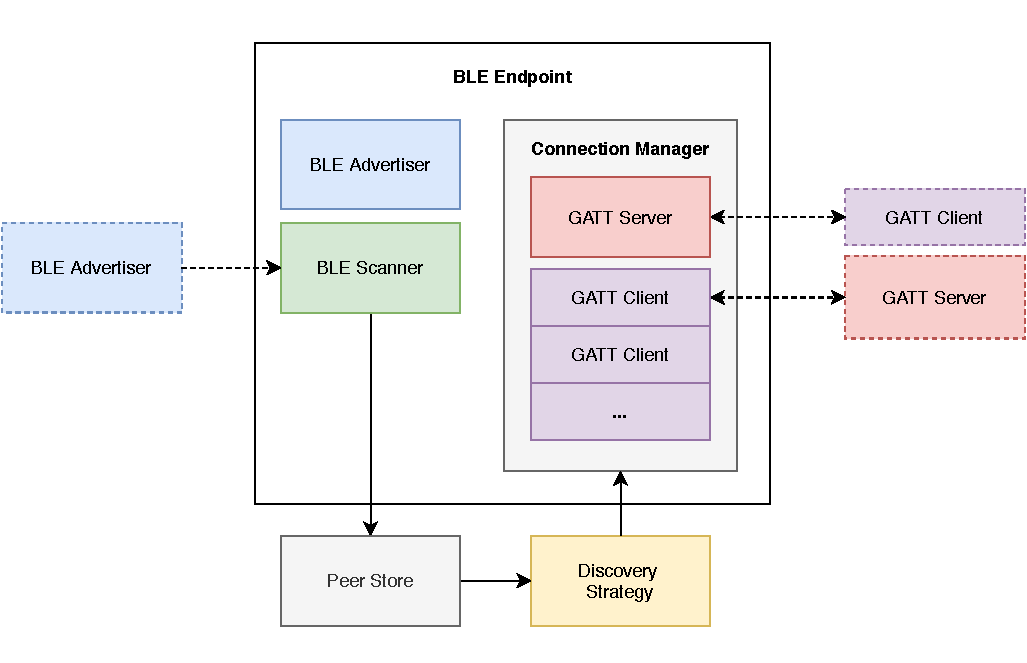
\includegraphics[width=\textwidth]{diagrams/ipv8-ble-architecture}
    \caption{Bluetooth Low Energy Communication Architecture}
    \label{ble_architecture}
\end{figure}

The BLE module should be composed of several submodules with clearly separated responsibilities. The communication begins by the device A broadcasting connectable advertising packets using \textbf{BLE Advertiser}. The advertising packet contains:

\begin{itemize}
    \item a \textit{service UUID} which identifies our application,
    \item a \textit{transmission power level} in dB which can be used by the receiver to calculate a path loss and estimate the distance between devices, and
    \item a \textit{peer ID} which identifies the broadcasting device.
\end{itemize}

The device B then scans for advertising packets using a \textbf{BLE Scanner}. It should filter packets by service UUID to receive only packets relevant to our application. The BLE scan is a power-intensive operation, so it should be performed only when the user actually wants to connect to a new device. It could be done e.g. only when the application is in the foreground. In case we are designing a long-running service that should run in the background, a scan should be run periodically. We should have an option to specify a scan window duration and an interval between individual scans.

Once the scanner receives an advertising packet, it creates a \textit{peer candidate} which consists of a peer ID, a Bluetooth device address which can be used to initiate a connection, a transmission power level in dB, and a received signal strength (RSSI) in dBm. It stores the peer candidate into the \textbf{Peer Store}.

The \textbf{Discovery Strategy} is responsible for selecting which peer we should connect to. The strategy should be application-specific and can e.g. prefer to connect to devices with the largest RSSI value, or to connect only to known peers based on their peer ID. Once the strategy selects a peer it wants to contact, it is sent to the \textbf{Connection Manager}.

The connection manager contains all GATT-related communication logic. Each device has exactly one GATT server and an arbitrary number of GATT client instances, one for each device it is connected to. The GATT server implements a single GATT service containing two characteristics which are shown in Figure \ref{gatt_server}. The \textbf{Public Key} characteristic has a \textit{readable} permission and simply contains a public key of the peer. It is used to determine the identity of the device when initializing the connection and can be used for authentication and encryption in the further communication. The \textbf{Writer} characteristic with a \textit{writable} permission is then used for sending data from the client to the server. As we want to support bidirectional communication, every two devices need to have a pair of client–server and server–client connections. This can be implemented in a way that every time a GATT server receives an incoming connection, the connection manager initiates an outgoing connection to the GATT server of the connecting device. Only after both links are established, the connection is considered ready.

\begin{figure}
    \centering
    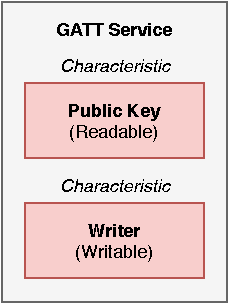
\includegraphics[width=0.25\textwidth]{diagrams/ipv8-gatt}
    \caption{Our GATT Server Architecture}
    \label{gatt_server}
\end{figure}

% GATT - service, characteristic, descriptor
% Service IPv8
% Characteristics
% - Member ID, permission read
% - Writer, permission write
% Handshake
% - 1. Read Member ID
% - 2. Wait for other peer to read our Member ID
% - 3. Send data to peer via its Writer

% Future Work:
% - L2CAP connection oriented channels (Android 10+)

% https://medium.com/@martijn.van.welie/making-android-ble-work-part-3-117d3a8aee23
% https://stefanbossbaly.com/2018/08/06/ble-in-android
% https://blog.classycode.com/a-short-story-about-android-ble-connection-timeouts-and-gatt-internal-errors-fa89e3f6a456
% https://punchthrough.com/android-ble-development-tips

\section{Relay Protocol with Bandwidth Accounting}

\chapter{Implementation}

% Android vs. iOS, interoperability
% Kotlin, Multiplatform - JVM + Android, but can be compiled to Native for iOS as well
% Android Things – IoT

\section{Project Structure}

% JVM vs. Android
% unit tests, TODO: Android tests
% library vs. super app separation

\section{System Architecture}

\subsection{Communities}

\subsection{Discovery Strategies}

\subsection{Endpoints}

\section{TrustChain: Scalable Accounting Mechanism}

% \section{Bluetooth Low Energy}

\section{Bootstrap Server}

%\section{Bluetooth Ad-Hoc Network}
%\subsection{Bluetooth Low Energy}
%\subsection{Generic Attribute Profile}

%\section{Multi-Transport Routing Algorithm}

%\section{Peer Discovery and Traversal in Distributed Hash Table}

%\section{Packet Format}

\section{Maintaining Backward Compatibility}
% continuous improvement while maintaining backward compatibility with 10 year old ipv8 implementation

\section{TrustChain Explorer}

%\section{Binary Transfer over UDP}

\section{PeerChat: Distributed Messenger}

%\section{Testbed for Distributed Android Applications}

\section{DelftDAO: Framework for Permissionless Economic Activity}

\chapter{Experiment}

\section{Analysis and Puncturing of Carrier Grade NAT}

According to the report by Statista \cite{statista:marketshare}, there were three major mobile phone operators providing services in the Netherlands in Q4 2018. They are listed in Table \ref{table_marketshare}. In total, these represent up to 85 \% of the market share. The rest of the market is shared by Mobile Virtual Network Operators who sell services over existing networks of those three operators.

\begin{table}[h!]
    \centering
    \begin{tabular}{ | l | c | }
        \hline
        \textbf{Operator} & \textbf{Market share} \\
        \hline
        KPN & 35\% \\
        Vodafone & 25\% \\
        Mobile Virtual Network Operators & 25\% \\
        T-Mobile & 20\% \\
        \hline
    \end{tabular}
    \caption{Market share of mobile network operators in the Netherlands in Q4 2018. The shares do not sum up to 100\% as they are rounded up within five percent ranges in the original report. \cite{statista:marketshare}}
    \label{table_marketshare}
\end{table}

We have purchased pre-paid SIM cards for all three major mobile network operators to investigate whether they are suitable for peer-to-peer communication. First, we tried to infer the characteristics of their Carrier Grade NAT deployments.

We used the STUN protocol and NAT behavior discovery mechanisms described in \cite{rfc5780}. They have shown that all networks appear to use \textit{Endpoint-Independent Mapping (EIM)} and \textit{Address and Port-Dependent Filtering} (also known as \textit{port-restricted cone NAT}). EIM is a sufficient condition for our NAT traversal mechanism to be successful, so this would make all these NATs suitable for P2P communication.

However, as NAT behavior can change over time, we performed some more tests to verify that the behavior is consistent over time. We attempted to connect to 50 different peers over the interval of 5 minutes. We verified that KPN and T-Mobile networks are consistent with EIM behavior. However, the Vodafone network changes the mapped port for new connections approximately every 60 seconds, even when connecting to the same IP address and a different port. This behavior can be described as \textit{Address and Port-Dependent Mapping}, which is characteristic for a \textit{symmetric NAT}.

The mapped ports seem to be assigned at random from the range of 10,000 ports, which makes it infeasible to use any known symmetric NAT traversal techniques such as port prediction or multiple hole punching \cite{multihole}\cite{takeda}.

%The results are presented in Table \ref{table_cgnat_analysis}.

\iffalse

\begin{table}[h!]
    \centering
    \begin{tabular}{ | l | l | l | l | }
        \hline
        \textbf{Operator} & \textbf{Mapping behavior} & \textbf{Filtering behavior} & \textbf{Binding lifetime} \\
        \hline
        KPN & Endpoint-Independent & Address and Port-Dependent & ? \\
        Vodafone & Endpoint-Independent / Address and Port-Dependent & Address and Port-Dependent & ? \\
        T-Mobile & Endpoint-Independent & Address and Port-Dependent & ? \\
        \hline
    \end{tabular}
    \caption{Characteristics of CGNATs deployed by Dutch mobile network operators}
    \label{table_cgnat_analysis}
\end{table}

\fi

% Types of NAT used by different operators
% - T-Mobile - Address-restricted cone
% - Vodafone – symmetric NAT, random port mapping, TODO: analyze port distribution
% - KPN - Address-restricted cone

%\section{Performance Evaluation}

\section{Bootstrap Performance Evaluation}

\section{Stress Test}

% experiments:
% - bootstrap from 0 to 20 peers
% - 24-hour stress test


\chapter{Conclusion}

\section{Future Work}
% IPv6 support, multiple network interfaces
% BLE mesh network
% Wi-Fi Aware for higher bandwidth Nearby transfer


%\input{2-state-of-the-art}

%\input{3-design}

%\input{4-implementation}

%\input{5-conclusion}

%% Use letters for the chapter numbers of the appendices.
\appendix

%\input{appendix-a}

\bibliography{references}

\end{document}

